\documentclass[
        a4paper,     % Format A4
        titlepage,   % mit Titelseite
        parskip      % mit Durchschuss
                     % (= Abstand zwischen Absätzen, statt Einrückung)
        ]{scrartcl} % KOMA-Script Grundklasse     texdoc scrguide

\usepackage[USenglish]{babel}
\usepackage[T1]{fontenc}          % Schriftkodierung mit Umlauten
\usepackage{textcomp,amsmath}     % Mathezeichen etc.
\usepackage{graphicx}             % Graphiken einbinden
\usepackage[utf8]{inputenc}				% direkte Eingabe von Umlauten & Co. (Vorsicht: Encoding im Editor muss auch UTF-8 sein!)

% bibtex
\usepackage{url}
\bibliographystyle{plaindin}      % BibTeX Styles nach Norm DIN 1505

\renewenvironment{abstract}[1]
% https://tex.stackexchange.com/questions/151583/how-to-adjust-the-width-of-abstract
 {\small
  \begin{center}
  \bfseries #1\vspace{-.6em}\vspace{0pt}
  \end{center}
  \list{}{
    \setlength{\leftmargin}{.6cm}%
    \setlength{\rightmargin}{\leftmargin}%
  }%
  \item\relax}
 {\endlist}

\newcommand{\sign}[1]{
	%https://tex.stackexchange.com/questions/183698/signature-line-with-dots-and-name-below      
  \begin{tabular}[t]{@{}l@{}}
  \makebox[2.5in]{\dotfill}\\
  \strut#1\strut
  \end{tabular}
}
\titlehead{

\includegraphics{Graphics/hpi_logo_cmyk_wb_sl2}
} \subject{Bachelor Thesis}
\title{Feature Extraction for Business Entity Linking in Newspaper Articles
\\ \bigskip 
\large{Merkmalsextraktion zur Unternehmenserkennung in Zeitungsartikeln}}
\author{Jonathan Janetzki\\{\small{\url{jonjanetzki@gmail.com}}}}
\date{\today}
\publishers{
Information Systems Group\\
~\\
\textbf{Supervisors}\\
Prof. Dr. Felix Naumann\\
Toni Grütze\\
Michael Loster}


\begin{document}
\maketitle

\newpage
\begin{abstract}{Abstract}
German newspaper articles contain a lot of recent information about business relations. Their automated retrieval allows to construct the \textit{German Corporate Graph} and keep it up to date. This can be done by means of NER and NEL to find the mentioned businesses. Since business aliases may be ambiguous, this is a complex problem. Its solution requires the extraction and comparison of expressive features for business entity linking.

This research work comprises a software system that finds and disambiguates references to organizations in newspaper articles by means of appropriate features. It uses the German Wikipedia that contains explicit link annotations to named entities and learns from it to recognize mentions of organizations. The extracted features are statistical measures, linguistic properties of the alias' context and second order features. The system then applies these features to newspaper articles without link annotations, which allows to find business aliases and their referenced entities.

The distributions of the features' values reveals that they strongly depend on whether a reference is valid or not. This means that the features have a high quality and are applicable by a classifier. Furthermore, the software is scalable in order to be also suitable for economical use on large amounts of data. 
\end{abstract}

\newpage
\begin{otherlanguage}{ngerman}
\begin{abstract}{Zusammenfassung}
Deutsche Zeitungsartikel enthalten eine Menge aktueller Informationen über Unternehmensbeziehungen. Ihre automatische Extraktion ermöglicht es, den \textit{Deutschen Unternehmensgraphen} zu konstruieren und auf dem neusten Stand zu halten. Dies kann mithilfe von NER und NEL erreicht werden, um die genannten Unternehmen zu finden. Da Unternehmensnamen mehrdeutig sein können, ist dies eine komplexe Aufgabe. Ihre Lösung erfordert die Extraktion und den Verleich von aussagekräftigen Merkmalen zur Unternehmenserkennung.

Diese Forschungsarbeit umfasst ein Softwaresystem, das Verweise auf Organisationen in Zeitungsartikeln mithilfe von angemessenen Merkmalen eindeutig ermittelt. Es benutzt die deutschsprachige Wikipedia, die explizite Linkannotationen auf benannte Entitäten enthält, und lernt daraus, Nennungen von Organisationen wiederzuerkennen. Die extrahierten Merkmale sind statistische Maße, linguistische Eigenschaften des Kontexts eines Alias' und Merkmale zweiter Art. Das System wendet diese Merkmale dann auf Zeitungsartikel ohne Annotationen an, was das Finden von Unternehmensnamen und ihren referenzierten Entitäten ermöglicht.

Die Verteilung der Merkmalswerte zeigt, dass diese stark davon abhängen, ob eine Referenz gültig ist oder nicht. Das heißt, dass die Merkmale eine hohe Qualität besitzen und von einem Klassifikator verwendet werden können. Darüber hinaus ist die Software skalierbar, um auch für große Datenmengen wirtschatlich einsetzbar zu sein.
\end{abstract}
\end{otherlanguage}
\newpage
%{\small\tableofcontents}
\tableofcontents
\addtocontents{toc}{\setcounter{tocdepth}{2}}
\newpage
\section{The German Corporate Graph Project}
\label{sec_project}

\subsection{Why a German Corporate Graph?}

When it comes to economic decisions, uncertainty is a critical issue. Following the approach of the rational choice theory, every market player is constantly trying to maximize his utility and to minimize his effort.

Uncertainty can be described as a lack of information of how a market - or here in the full German economic system - is constituted and about the future behavior of the market players. Presuming that every market player is acting on a rational basis, every information regarding his situation, resources, plans, and relations makes the results of his decisions more predictable. In this manner, we can state: The more relevant information a market player gathers about other players in the market or economy, the better the foundation of his decisions are. The broad range of that kind of information can lead to a significant competitive advantage. So it should be in a rational player's interest to collect as much relevant information as possible.
\medskip

In a connected economy, a lot of those uncertainties lay in the relations between corporations\footnote{We define as \emph{corporation} any juristic entity that takes part in the German economy. This includes especially businesses but also other entities like public corporations.}. This became evident in the so called \emph{Abgas-Skandal} or \emph{Dieselgate} of the Volkswagen AG in 2015, wherein a lot of external suppliers went into a spin, from a financial perspective \cite{stuttzeit}, \cite{automobilwoche}. This happened although most of the suppliers did not take part in the scandal itself. Since there are a lot of other examples like the \emph{Lehmann Brothers bankrupt} or any other kind of economic shock event, we can state that relations are a significant factor in the economic evaluation of corporations and their financial risks.
\medskip

Because there are millions of corporations in the German economy\footnote{ The \emph{Federal Bureau of Statistics} is noting 3,469,039 businesses in Germany in 2015 \cite{destatis1}. Following our definition of corporations, this number has to be seen as a lower bound for the total number of corporations in Germany.} and each corporation can potentially holding relations to hundreds or thousands of other corporations, the aim to collect and to overview all those relations becomes a complicated matter.
\medskip

This is where the \emph{German Corporate Graph Project} offers IT-based solutions. The project\grq s purpose is to explore and evaluate ways, methods, and obstacles on the journey from collecting information about relations to transform them into a graph representation on a big scale. Therefore the project participants developed a software pipeline. 
\newpage
This software pipeline covers the following steps and components:
\begin{itemize}
\item Normalization of attributes to a common shape
\item Automatic graph generation from structured data sources
\item Deduplication: Duplicate detection and data-fusion 
\item Information extraction: NEL and NER on semi-structured and unstructured data sources
\item Curation interface: A web interface to control the whole pipeline, to aggregate pipeline statistics and to curate graph data by hand
\item Corporate Landscape Explorer: A web interface to explore the \emph{German Corporate Graph} visually   
\end{itemize}


\subsection{One project - seven contributions}

This thesis is published as a part of a bachelor\grq s project in 2016/2017 at Hasso-Plattner-Institute in Potsdam, Germany. The project\grq s objective was to build the \emph {German Corporate Graph}, like described above, for Germany\grq s corporate landscape. The project lasted ten months and was accompanied by Commerzbank AG, Germany. As a result, the project participants published several theses. 



See here a list of all published theses within the project\grq s context:

\begin{itemize}
\item Pabst explores \emph{Efficient Blocking Strategies on Business Data} \cite{pabst}.
\item Löper and Radscheit evaluate duplicate detection in their thesis \emph{Evaluation of Duplicate Detection in the Domain of German Businesses} \cite{loeperradscheit}.
\item Schneider\grq s thesis is entitled \emph{Evaluation of Business Relation Extraction Methods from Text} \cite{schneider}.
\item Janetzki investigates \emph{Feature Extraction for Business Entity Linking in Newspaper Articles} \cite{janetzki}.
\item Ehmüller explores the \emph{Evaluation of Entity Linking Models on Business Data} \cite{ehmueller}.
\item \emph{Graph Analysis and Simplification on Business Graphs} is the title of Gruner\grq s thesis \cite{gruner}.
\item Strelow investigates the \emph{Distributed Business Relations in Apache Cassandra} \cite{strelow}.

\end{itemize}
~\\
\section[Ambiguous Business Aliases]{Ambiguous Business Aliases\protect\footnote{This section was written in collaboration with Jan Ehmüller~\cite{ehmueller}.}}
\label{sec:introduction}
The graph of Germany's corporate landscape consists of businesses as nodes and their relations as edges. Although structured knowledge bases, such as Wikidata and DBpedia, provide extensive information, they miss information about the relations. These are described in unstructured texts like Wikipedia or newspaper articles.

We have developed an approach to extract a relation between two businesses if they are mentioned in the same sentence. Then both of these mentions need to be found and linked to the entities representing these businesses. Finding these mentions is called \textit{Named Entity Recognition} (NER). The next step is to link them to the correct entity, which is called \textit{Entity Linking} (EL). The eventual extraction the relation between these two businesses from the sentence is called \textit{Relation Extraction} (RE). Our approach combines NER and EL into a single process and reduces it into a classification problem. The combination of NER, EL and RE make up the Information Extraction component of our project.

This thesis focuses on the development of a reliable implementation for combined NER and EL. Since there is no one-to-one relationship between businesses and their aliases, this is a complex task. On the one hand, a business may have multiple aliases. For example, "Deutsche Bahn AG" is commonly abbreviated with "Deutsche Bahn" or simply "DB". On the other hand, aliases are ambiguous, which means that the same alias may refer to different businesses in different contexts. This holds true especially for abbreviations. For example, "DB" may also refer to "Deutsche Bank AG". We therefore extract expressive features that allow us to disambiguate such business aliases and link them to their actually meant entity.

Sec.~\ref{sec:related_work} covers related work in the field of both NER and EL. Sec.~\ref{sec:ner_el} explains how our combined NER and EL approach works, before Sec.~\ref{sec:features} characterizes which features we use to perform EL. Sec.~\ref{sec:preprocessing} then describes our data sources and how they are used for the feature extraction. After that, Sec.~\ref{sec:evaluation} discusses the quality of the features and the scalability of the implementation. Finally, Sec.~\ref{sec:conclusion} will summarize the results and what steps may improve the project in the future.

~\\
\section{Related Work}
\label{sec:related_work}
Various research teams have worked on projects, which aimed on automatically linking aliases from natural language text to German businesses as well. The following outline gives an overview about what they already have attained:

\subsection{Alias generation to improve company recognition in text}
Alexander Immer has worked on the bachelor project previous to this project~\cite{immer}. Starting from legal names, he researched how aliases can be generated by abbreviating and pruning them. To disambiguate ambiguous aliases, he uses two vector spaces: One for the tf-idf values of words occurring in the neighborhood of recognized aliases and another one for words occurring in newspaper articles in general. He achieved an f-score of 0.81 for the named entity recognition on German newspaper articles and an f-score of 0.79 for named entity linking. Our approach also uses two different vector spaces, but they are constructed in another way. In contrast to Alexander's system, we do not generate aliases by ourselves, but we retrieve them from the German Wikipedia.

\subsection{The CohEEL project}
The CohEEL project attempts to perform named entity recognition and named entity linking on natural language texts for general purposes~\cite{coheel}. Like our system, it also uses the features link score, page score and context score that are described in Sec.~\ref{sec:features}. We go a step further and also include second order features that are retrieved from those features and support the classifier.

\subsection{Stanford CoreNLP}
The Stanford CoreNLP has a component for named entity recognition that detects mentions of organizations in natural language texts~\cite{stanford}. In contrast to our approach, it uses a neuronal network (?). Also it does not link the recognized mentions to specific organizations, it yields comparable results regarding the NER.
~\\
\section{Joint NER and EL in Newspaper Articles}
\label{sec:ner_el}

Newspaper articles contain a lot of current information about business relations. E.g., a German article might contain a sentence like: "Bosch liefert Servomotoren an die DB." (English: "Bosch delivers servo motors to the DB.") For a human it is obvious that this sentence represents a delivery relation between the entities: "Robert Bosch GmbH" and "Deutsche Bahn AG". While "DB" could also abbreviate "Deutsche Bank" [todo: AG?], the technical context makes clear that the railroad company (?) is meant instead of the bank.

As such relations are useful for our business graph, we want to extract those from free text, such as newspaper articles. In order to do so, we need to perform joint NER and EL beforehand. This section describes how we identify which businesses are mentioned in free texts.\\

\subsection{Newspaper data sources}
Currently, we perform joint NER and EL on the German Wikipedia and the German newspaper Spiegel Online [todo: link]. As Wikipedia already contains links to named entities, we use it as training data (see Sec.~\ref{sec:pipeline}) and ground truth for the evaluation [todo: reference jan]. Newspaper articles are missing such annotations.

For Spiegel Online, we use a dump that consists of HTML, contains 260000 articles (?) and has a total size of (?) GB. On (?) average, the text of each article consists of (?) characters.\\

\subsection{Process}
The joint NER and EL consists of multiple steps, as depicted in Fig.~\ref{fig:ner_el_process}. Apart from the data import, the steps are independent from the data source so that they can be reused easily.

\begin{figure}[ht]
	\centering
  \includegraphics[width=\textwidth]{Graphics/pipeline.pdf}
	\caption{Steps of the joint NER and EL process}
	\label{fig:ner_el_process}
\end{figure}

\subsubsection{Data import}
For each article, the Spiegel Online dump provides the title, the text and a unique internal ID. We extract these three values from the dump and store them in a Cassandra table. As the German Wikipedia dump provides similar information, we store it in a table with the exact same format. The only difference to Spiegel Online is that the title of an article already is a unique ID.\\

\subsubsection{Potential named entity recognition}
A mention of a named entity in a text is a chain of one or more consecutive tokens, where a token is a semantic element of a text. This is a word in most cases, but can also be a special character, such as a comma. The task of named entity recognition is to identify such chains in text. This step is important for our process, as EL needs to be performed on a pre-selection of those. Otherwise it would have to try to link each n-gram in the text to a named entity, which would lead to a computational complexity that increases exponential with the number of tokens. This would be inacceptable for our task.

[todo: Example with comma]

But in contrast to NER, we create a larger pre-selection of potential named entities that may signify a named entity depending on the context. This step is therefore called "potential named entity recognition". It is much easier than NER, as EL will decide to which named entity a named entity candidate links, which is a very similar task to deciding whether it links to a named entity at all. In our case, this is what EL will do later on.

We find candidates of named entities simply by selecting all those token chains that were named entities of organizations within the training data (see Sec.~\ref{sec:alias_analysis}). An efficient way to match those is by means of a trie, which we implemented as a token based prefix tree.\\

[todo: explain logarithmic time]


\subsubsection{Feature extraction}
Before we can perform EL on the link candidates, we need to extract features from them that are characteristic for links to specific targets. Inspired by the CohEEL project~\cite{coheel}, we decided to use three features: The link score, the entity score and the context score. Section~\ref{sec:features} describes them in detail.

We extract all these features for each link candidate. As we have a lot of explicit link annotations [todo: number] in Wikipedia, we also extracted these features from those links as well as from occurrences of organization aliases that do not signify an organization so that we have comparable labeled data.\\


\subsubsection{Entity Linking}
By means of the labeled composite features and new ones extracted for each link candidate, we can reduce the task of EL to a classification problem: By training a classifier model with the ground truth data it can decide whether each link candidate links to an organization or not and if it does, to which. Ehmüller~\cite{ehmueller} describes how the classifier works in detail and which configurations leads to the best results.

Now we know where and which organizations are mentioned in a German newspaper article. Where a text mentions multiple organizations, it is likely that it describes a relation between those. Schneider~\cite{schneider} researched how we can extract those relations in order to enrich the \textit{German Corporate Graph}.\\


\subsubsection{HTML Export}
If the user of our generated \textit{German Corporate Graph} finds a business relation that is unexpected, or if they simply want to comprehend how it was retrieved, it is necessary to provide a reference to the respective part of the original newspaper article, if applicable. An additional visualization of how the relation was extracted makes this even more useful. In terms of the joint NER and EL process, we show where we have linked which tokens to which organizations. Therefore we enrich the original texts with HTML-links from the tokens to the Wikipedia article of their respective entity. We then export the HTML article to our Curation interface~\cite{gruner}, where the user can explore the results of the joint NER and EL process.\\

~\\
\section{Features for Business Entity Linking}
\label{sec:features}
We use certain features to describe chains of tokens in order to perform EL. On the one hand, they have to be expressive so that they allow us identify the correct businesses, on the other hand they have to be simple enough to be comparable for our classifier model. Inspired by the CohEEL project~\cite{coheel}, we use three features for each link candidate: The link score, the entity score and the context score. Each of them is a real number in the interval $[0, 1]$. The entity score and context score are enriched with additional second order features describing their proportion to "competing" values.



\subsection{Link score}
\label{sec:link_score}
The link score $ls$ of an alias $a$ is the probability that it links to a business inside our training data:

\begin{equation*} % *: suppress numbering
ls(a) = \frac{|\text{Occurrences of $a$ as link}|}{|\text{Total occurrences of $a$}|}
\end{equation*}

This feature is the most important for deciding whether a business alias signifies a business or not. For example, the alias "Bank" occurs 2200 times as a link but 44000 times for total. It may link to a certain organization, such as the German Sparda-Bank union. But in most cases, it denotes a bank in general or an ordinary bench, which is not linked in most cases. The low link score of 0.05 reflects that the alias "Bank" is not likely to denote a certain entity.\\



\subsection{Entity score}
\label{sec:entity_score}
As already mentioned, a business alias may signify different businesses in different contexts. For example "Telekom" occurs 700 times as a link and may refer to different businesses. In 450 cases it links to the "Deutsche Telekom AG" and in 140 cases to the "Telekom Deutschland GmbH", which is a subsidiary of "Deutsche Telekom".\footnotemark{} As our system has to be aware of this ambiguity, we introduce the entity score $es$ of an alias $a$ and an entity $en$ as a second feature. Provided that $a$ is a link to an entity, it is the probability that $a$ links to $en$ inside our training data:
\footnotetext{\url{https://www.telekom.com/de/konzern/weltweit/profile/die-deutsche-telekom-in-deutschland-336242}, last accessed on \formatdate{19}{7}{2017}.}

\begin{equation*}
es_{en}(a) = \frac{|\text{Occurrences of $a$ as link to $en$}|}{|\text{Occurrences of $a$ as a link}|}
\end{equation*}

For the alias "Telekom" this results in an entity score of 0.64 for the entity "Deutsche Telekom AG" and 0.20 for "Telekom Deutschland GmbH". [optional: Graphic] These values allow our EL step to prefer those businesses that are more likely than others.\\


\subsection{Context score}
\label{sec:context_score}
If our system would perform EL only based on the link score and entity score, it would never decide that an alias refers to an entity that has not the highest entity score for this alias. But depending on the context of an alias it may be clear that an entity with a low entity score is meant. [todo: Example] Therefore we need a comparable mathematical representation of an alias' context.


\subsubsection{Tf-idf contexts}
We consider the bag of words of respectively 20 preceding and successive tokens (if existing) as sufficient for the disambiguation of an alias. This model counts how often which token occurred and disregards grammatical dependencies. We also perform stemming, which means that we normalize the tokens by discarding their grammatical forms. This generalizes the context even further and makes it easier comparable to other contexts. Furthermore, we discard stop words that are very common in German texts and therefore considered as not representative. When we compare bags of words, we want that those words have a strong impact that are significant. The more a word occurs in a bag of words and the less it occurs outside it, the more it is considered as significant. This is a well-known requirement in the field of information extraction and commonly solved by means of the tf-idf measure. It describes the significance of a word as a single value greater than zero, based on its frequencies in a bag of words and the text corpus.

[todo: insert formula]

We use this measure to transform each bag of words into a vector of tf-idf values for each contained word. We call this vector the \textit{tf-idf context} of an alias. This numerical representation of a context is easy comparable to other tf-idf vectors.


\subsubsection{Cosine similarity}
To disambiguate an alias, we also compute a tf-idf vectors for each German Wikipedia article. We assume that an alias is likely to refer to an specific entity, when its tf-idf context is similar to the tf-idf vector of this entities' article, as they describe the same subject and probably use the same words. We therefore compute the similarity between both vectors. This is our third feature, the context score. We use the cosine similarity, which is a common approach to compare vectors:

[todo: insert formula]

~\\
While the link score and entity score are statistical features that have always equal values for each pair of an alias and an entity candidate, the context score makes the system capable of disambiguating an alias based on its surrounding text.



\subsection{Second order features}
When the classifier disambiguates an alias, it has a single link score and one entity score and context score for each entity candidate. As not more than one entity can be correct, the entity scores and context scores are "competing" against each other. As the classifier only makes a binary decision - whether an alias with a given context refers to a given entity or not - it cannot consider how likely the alternative entities are if the features are provided as they are.

Second order features are additional values for scores that represent the relation to such competing scores. By means of those, the classifier is able to consider, e.g., that an entity is likely for an alias, because it has the highest entity score, although it is smaller than 0.5.

For each entity score and the context score, we add the following second order features:

\begin{enumerate}
\item The \textbf{rank} $r$ is a natural number that denotes how many competing scores are greater than the respective scores (plus 1). It starts from 1 for the highest score(s).

\item The \textbf{absolute difference to the highest value} $\Delta top$ lies in the interval $(0, 1]$. The classifier should consider the highest score separately, what we achieve by using $+\infty$ instead of 0.

\item The \textbf{absolute difference to the next smaller value} $\Delta successor$ also lies in the interval $(0, 1]$. Here, the classifier should consider the smallest score separately, what we achieve by using $+\infty$ for it.
\end{enumerate}

In this way the entity score and context score both become tuples of their original value and three additional values.
~\\
\section{Text Mining Pipeline}
\label{sec:pipeline}
This section describes how the raw data is preprocessed in order to train a classifier that performs NER and EL on German newspaper articles.
~\\
Preprocesing on Wikipedia dump\\
Explanation of jobs and their runtimes\\
Tools: Stanford CoreNLP (Tokenizer), Apache Lucene (Stemmer)\\
Data structures: Trie (for alias recognition)\\

\subsection{Raw data}
The system uses Wikipedia and Wikidata as data sources to train the classifier that performs EL. The following will describe both of them.

\subsubsection{Wikipedia}
As project aims on analyzing German newspaper articles, the German Wikipedia provides appropriate training data. It currently consists of more than 3.6 million articles [source]. The articles have 3 main components:
\begin{itemize}
\item Natural language text makes up most of the data.
\item Links to other Wikipedia pages.
\item Structured content, such as infoboxes.
\end{itemize}
The system will train the classifier based on the text and the links. It discards the structured content, as most of it is part of DBpedia [source], which is already included in the company graph [source reference to other BA].\\
For faster processing, the system accesses this data via a dump of the Wikipedia [source link] that consists of XML and Wikimarkup. The whole dump has a size of 15.9 GiB.

\subsubsection{Wikidata}
The German Wikidata [source link] describes the same entities as the German Wikipedia. But in contrast to Wikipedia, it does not provide a textual description but an ontology for them. This includes the class of an entity, which can be a business or an organization [todo concrete identifier]. This information is used to train the classifier only with relevant data.\\
As Wikipedia, the system also accesses the German Wikidata via a dump that is stored as JSON. It has a size of 90.2 GiB.

\subsection{Overview}
The preprocessing of the raw data consists of multiple steps as depicted in Fig.~\ref{fig:job_dependencies}. The system
\begin{itemize}
\item filters the data sources for their relevant content and stores this into tables of an Apache Cassandra database. (Parsing)
\item refines the links within the Wikipedia and counts the references between each alias and entity. (Link analysis)
\item searches for aliases of organizations in the Wikipedia text. (Alias analysis) 
\item analyzes the frequencies of words in the Wikipedia text. (Word analysis)
\end{itemize}

In the following steps, the system
\begin{itemize}
\item generates features to train the classifier. (Feature generation)
\item trains the classifier. (Classifier training)
\item performs EL on newspaper articles. (EL)
\end{itemize}

\begin{figure}[ht]
	\centering
  \includegraphics[width=\textwidth]{Graphics/pipeline.pdf}
	\caption{Data sources of the text mining pipeline, steps (green) and the resulting Named Entity Classifier (blue)}
	\label{fig:job_dependencies}
\end{figure}


\subsection{Data preprocessing}
This subsection describes how the presented steps work in detail.

\subsubsection{Parsing}
For each article in Wikipedia, the parsing step converts the Wikimarkup to HTML by means of [source tool]. It then extracts the raw text and saves it into a Cassandra table along with the contained links to other Wikipedia entities.

\subsubsection{Link analysis}
At first, the link analysis step refines the extracted Wikipedia links. This means that it removes links to nonexistent pages and resolves links to redirect pages to their final target pages.\\
Secondly, the link analysis generates statistics about how often a specific alias occurs as a link and which target pages it has how often. For example, the alias "BMW" occurs 5700 times as a link, and directs in 4264 cases to the page "BMW". In only 6 cases, it directs to the page "Berlins Most Wanted". The link analysis also generates these statistics vice versa by counting how often a specific page is linked by which aliases. This means, for example, that the page "BMW" is linked by the alias "BMW" in 4264 cases but only 155 times by "BMW AG". [graphic for this example] These statistics are helpful to identify aliases of organizations, estimate the probability that an alias means an organization (see Sec.~\ref{sec:link_score}) and that it means a specific organization (see Sec.~\ref{sec:entity_score}).\\

\subsubsection{Alias analysis}
\label{sec:alias_analysis}
Most of the links [concrete number] that are contained in Wikipedia are not relevant for the desired company graph, as they do not link to an organization. Wikidata provides an ontology that allows to identify which of Wikipedia's entities is an organization. This could be used to discard all links that do not link to an organization. But instead, the alias analysis uses the statistic from the previous step that lists all occurring aliases for a specific page to find all aliases that link to an organization. Only after it has determined these aliases, the alias analysis removes all those links that have an alias that directs to an organization in no case. In this way, the system retains links that do not link to an organization but have an alias of an organization. Those links are a valuable true negatives that are used to train the classifier that identifies mentions of organizations in raw text later on [reference to classifier training].\\
To gain even more training data for the classifier, the alias analysis builds a trie (a token based prefix tree) that contains all known aliases. It then uses the trie to identify all occurrences of organization aliases in Wikipedia articles that are no links. The alias analysis assumes aliases that also occur as a link in the same article as meaning the same entity. It saves them as so-called extended links, which serve as true positives. If aliases have no corresponding link in the same article, the alias analysis saves them as a so-called trie hit, which serve as true negatives.\\

\subsubsection{Word analysis}
As an alias may have multiple meanings, the classifier requires additional information to disambiguate its occurrences in newspaper articles. A helpful feature is the context of those occurrences (see Sec.~\ref{sec:context_score}), since it strongly depends on their meaning. The classifier therefore needs a way to describe the content of raw text.\\
In NLP, a common approach to evaluate the content of raw text is the bag-of-words model [link]. This model considers a text as a multiset of its contained words, which means a set that may contain words multiple times. Although the order of the words is lost, the model can be used to determine whether different texts describe similar subjects or not. For example, two newspaper articles that contain the words "Automobil" (automobile) and "Ingolstadt" multiple times are likely to both address the German automobile manufacturer "Audi", as its headquarters are located in Ingolstadt.\\
As the last step of the data preprocessing, the word analysis step extracts those bag of words for each Wikipedia article and each context of a link or extended link. We assume that 20 words before as well as after the link occurrence are representative for the meaning of the alias. This bag of words is called the context of the link.\\

\subsection{Classifier training}
By means of the preprocessed data, the system extracts various features for named entities in text. It uses them to train a classifier model in order to recognize named entities in raw text without link annotations.\\

\subsubsection{Input and output}
For an alias within a text, the classifier decides whether it denotes a named entity or not. If it does, it specifies the respective named entity.\\
As we wanted to build on reliable implementations of existing classifier models, we implemented the classifier as a binary classifier that operates on numerical values. This means that the classifier may only distinguish between two classes. Applied to EL, the classifier's input is not only an alias, but also a concrete candidate for a named entity. It then decides whether the alias denotes this named entity or not.\\
The random forest classifier model seemed to be the most appropriate model for this application.\\
%todo: abgrenzen zu anderen classifier models, z.B. neuronale Netzwerke

\subsubsection{Random forest classifier model}
The classifier is a random forest classifier that is trained by means of the Spark MLlib, which is a library for distributed machine learning [source link]. A random forest classifier is a set of independently trained decision trees [source link]. Each of them makes a decision based on the given feature values. The classifier defines a decision function that depends on the number of trees that have made a respective decision. The easiest function is the majority vote.\\
There are multiple parameters that influence the structure and quality of the forest: In our case, it consists of five trees at maximum and has not more than 32 bins per tree.\\
~\\
The next section describes the features for the classifier in detail.
~\\
\section{Evaluation}
\label{sec:evaluation}
Our system needs be suitable for economical use. This can be expressed as two requirements: On the one hand, the found joint NER and NEL process should find as many correct references as possible to organizations. While Ehmüller~\cite{ehmueller} evaluates this in terms of the standard measures precision, recall and $F_1$ score, we focus on how significant the features are without considering a certain classifier model. On the other hand, our system has to be capable of processing large amounts of data in reasonable time. As our project aims on solving this by means of cluster computing, we evaluate how well the described preprocessing scales out.



\subsection{Significance of the features}
Given a link candidate $lc=(a, c)$ consisting of an alias $a$ and its context $c$ and an entity $en$, the classifier decides whether $lc$ references $en$ or not. Note that, while the link candidate's entity score $es_{en}(a)$ and the context score $cs_{en}(c)$ depend on $en$, $ls(a)$ only depends on the alias itself. Therefore these features must allow a distinction between valid and invalid links regarding the given entity. In the following, I evaluate the distribution of the features based on a sample of 100,000 composite features and how expressive they are for this distinction.

\begin{figure}[h]
	\begin{tabular}{cc}
	\subfloat[Composite distribution of the entity score and the context score]{
		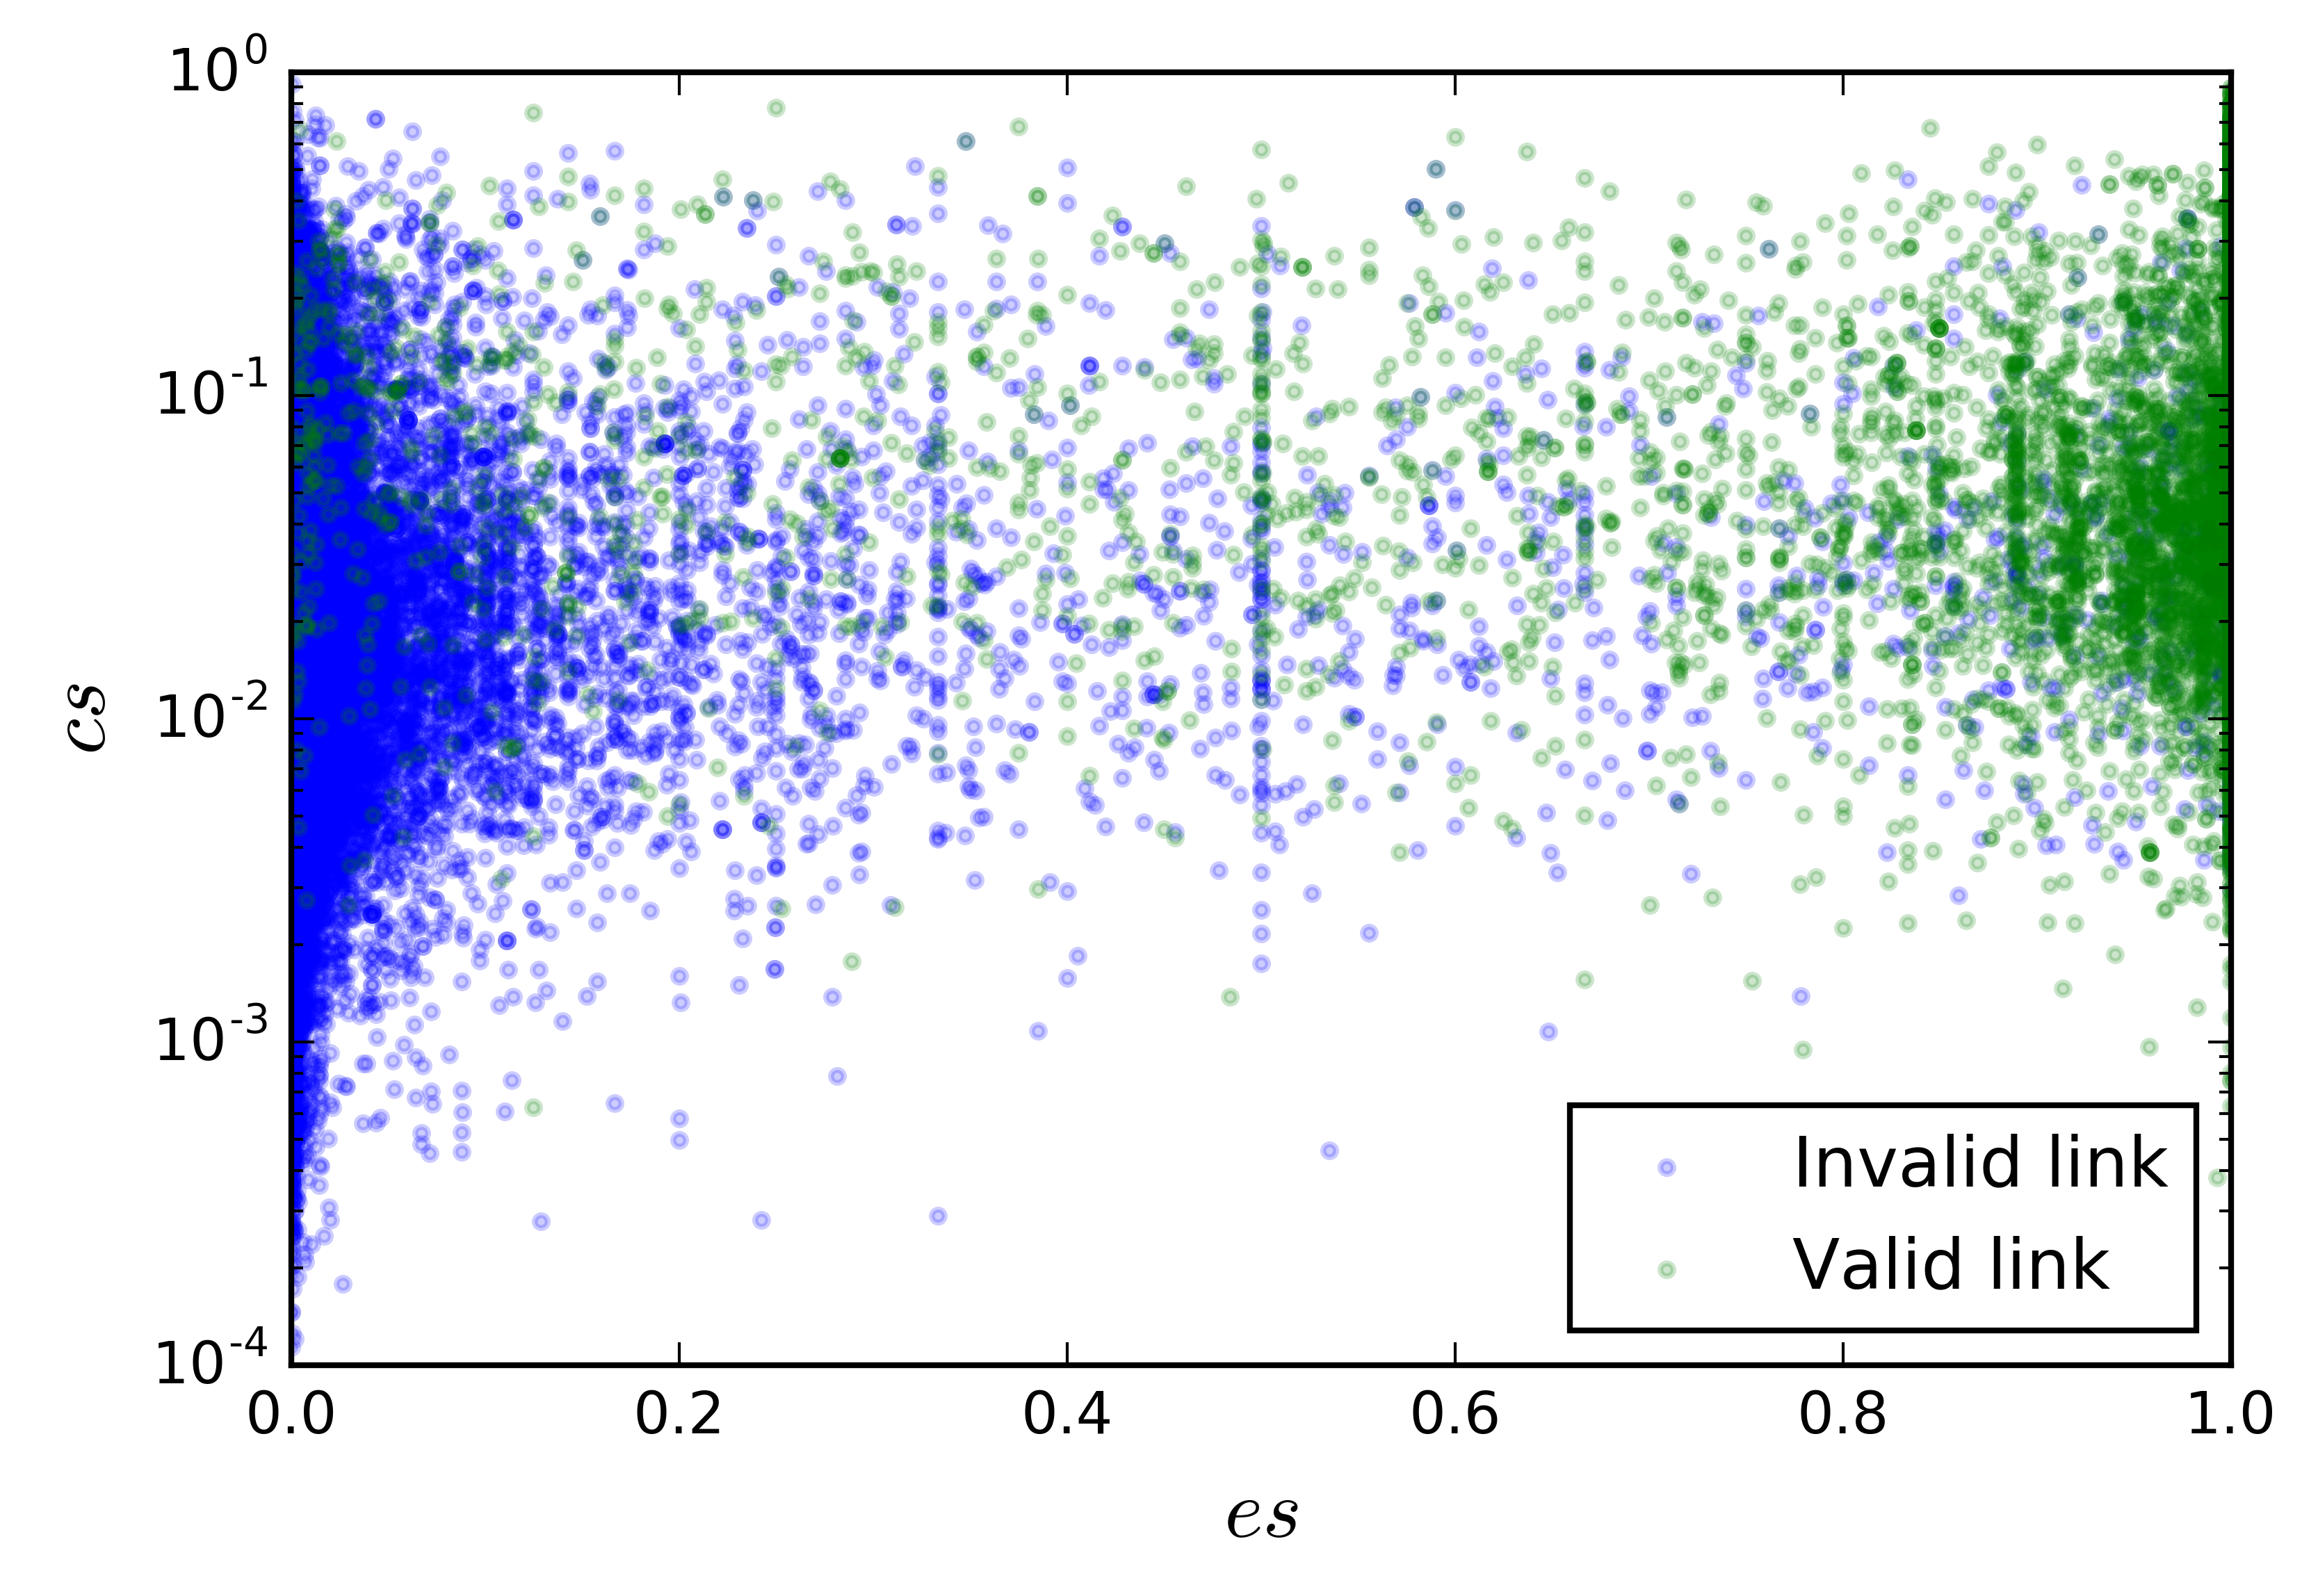
\includegraphics[width = 0.45\textwidth]{Graphics/feature_evaluation/composite_features.png}
		\label{fig:composite_features}
	} &
	\subfloat[Distribtion of the link scores]{
		\includegraphics[width = 0.45\textwidth]{Graphics/feature_evaluation/link_scores.pdf}
		\label{fig:link_scores}
	}\\
	\subfloat[Distribtion of the entity scores]{
		\includegraphics[width = 0.45\textwidth]{Graphics/feature_evaluation/entity_scores.pdf}
		\label{fig:entity_scores}
	} &
	\subfloat[Distribtion of the context scores]{
		\includegraphics[width = 0.45\textwidth]{Graphics/feature_evaluation/context_scores.pdf}
		\label{fig:context_scores}
	}
	\end{tabular}
	\caption{The three used features have significantly different distributions for valid and invalid links.}
	\label{fig:distributions}
\end{figure}

Figure~\ref{fig:composite_features} gives an overview about the composite distribution of the entity score and context score. Note that the context score is scaled logarithmically. The diagram reveals three properties:

\begin{enumerate}
\item There are two clearly identifiable \textbf{clusters}: One for valid links and a high entity score and one for invalid links and a low entity score. 

\item The entity score is more expressive than the context score, as the clusters can only be separated by means of the entity score.

\item There is a \textbf{correlation} between the entity score and the context score: There are far more valid links in the upper right half than in the lower left half of the diagram. This means, that the entity score and context score are "`confirming"' each other.
\end{enumerate}

Now we consider the features separately to get a more concise understanding of their quality:

\paragraph{Link score}
Figure~\ref{fig:link_scores} shows the distribution of the link scores for the valid and invalid links. Here and in the following, the overlap between the bars is shaded in dark blue. As not more than one entity is valid for each link candidate, our sample contains only 8\% valid links. Thus, for the better visibility, $f$ shows the relative frequency that is 1 both for the valid and invalid links if added up. We can see that a valid link has a link score that is close to 1 in more than 60\% of cases, while invalid links have a link score that is widely distributed. In fact, almost all of the links represented by the last bar have a link score, which is exactly 1. This means, that there are a lot of explicit aliases, which always refer to the same entities. 

\paragraph{Entity score}
Figure~\ref{fig:entity_scores} shows the distribution of the entity scores. he extreme left and extreme right bar represent the clusters observed in Figure~\ref{fig:composite_features}. Thus, the entity score is very expressive for our task. A classifier that decides based on a linear separation between these clusters should yield reasonable results. But since the of valid links is relatively small, this feature is not sufficient.

\paragraph{Context score}
Finally, figure~\ref{fig:context_scores} shows the distribution of the context scores. Note that the frequency is scaled logarithmically. Although there is a large overlap between the valid and the invalid links, the distribution of the valid links is significantly shifted to higher context scores. For a context score of about 0.1, the context score has the least significance. The smaller or higher it becomes from there, the better the classifier can make its decisions.

\paragraph{Second order features}
Also the second order features have a high expressiveness, as shown in Figure~\ref{fig:second_order_features} in the appendix. Similar to the three features described above, they show significantly different distributions for valid and invalid links. Combined with them, the classifier improves the results of our NEL even further.


\subsection{Scale out}
\begin{figure}[ht]
	\centering
  \includegraphics[width=\textwidth]{Graphics/ReducedLinkAnalysis2.pdf}
	\caption{Scale out of the link analysis step}
	\label{fig:scale_out}
\end{figure}

In order to make our system scalable for arbitrary input sizes, we use the cluster computing framework Apache Spark\footnotemark{}. As an example for our scale out, Figure~\ref{fig:scale_out} shows the efficiency of our link analysis for a sample of 1,000,000 Wikipedia articles. The efficiency is computed as the average amount of articles that is processed within a second. The scale out was measured for a different number of nodes (i.e., physical computers) and a constant number or CPU cores. A linear scale out would be theoretically perfect. This means that the efficiency increases in the same proportion as the number of nodes. Since there is always communication overhead between the nodes, which increases runtimes, a linear scale or even super-linear scale out is hard to achieve. As we can see, we have an approximately linear scale out for two nodes, but overall, the scale out is sub-linear. The stagnancy for eight nodes might be explained by the relatively small input sample, which leads to an relatively higher communication overhead. The other steps of our preprocessing have similar scale outs.
\footnotetext{\url{https://spark.apache.org/}, last accessed on \formatdate{20}{7}{2017}.}

To contextualize our approach, we compare our approach to a common other implementation for standardized subtasks. This is possible for the computation of the link candidate contexts, which includes the extraction of the bags of words and the subsequent computation of the tf-idf vectors (see Sec.~\ref{sec:context_score}). An alternative implementation is part of the Spark MLlib\footnotemark{}, which was especially designed for cluster computing. 15 runs of both implementations for all links of the German Wikipedia led to an average time of 9.53 minutes for the Spark MLlib and 6.46 minutes for our approach. Therefore, it computes the contexts of link candidates 1.47 times faster than the Spark MLlib.
\footnotetext{\url{https://spark.apache.org/mllib/}, last accessed on \formatdate{20}{7}{2017}.}

~\\

As shown above, the features we use for the extraction of business relations from text have a high quality. They allow a distinction between valid and invalid references to entities. Furthermore, our preprocessing is suitable for cluster computing. It can be distributed over multiple nodes and has an increasing efficiency for a higher amount of computing resources.
~\\
\section{Conclusion and Outlook}
\label{sec:conclusion}
Ambiguous business aliases make business entity linking in newspaper articles a complex problem. It becomes possible by the extraction of expressive features, what we achieved by using statistical features, a linguistic feature and additional second order features. All of them turned out to have a significant correlation to whether an alias in a text refers to a certain business entity or not. We therefore used them to perform combined NER and EL to determine where a newspaper article mentions which businesses. Thanks to this disambiguation of business aliases, we were able to analyze newspaper articles even further and extract business relations from them. We then inserted them into the German Corporate Graph that helps to get a better understanding of the German corporate landscape.

Starting with this full operative system, the next steps would be more focused on adding more data sources and testing more features.

The most promising improvement is to expand the training data. So far, we only used the German Wikipedia and Wikidata. But these do by far not cover all German businesses. Additional structured data sources, such as Implisense, would provide more business aliases. Those can be used to detect even more of their mentions in texts. Besides, we only used Spiegel Online to perform combined NER and EL. To extract more business relations, we should include other German newspapers with an economical focus, such as heise online\footnotemark{}.
\footnotetext{\url{https://www.heise.de/}, last accessed on \formatdate{20}{7}{2017}.}

Since many businesses do not have a Wikipedia article or only few distinctive words in it, the enrichment of their tf-idf vectors would help to disambiguate aliases in a text. More of those words may be retrieved from, e.g, the homepage of the business or an article about its location. As some words are typical for an entire business sector, such as "Motor" for the automobile industry, tf-idf vectors can be generated from multiple articles regarding the same sector. These vectors can then be used for businesses without an article.

It is also advisable to disambiguate aliases based on other decisions inside the same newspaper article. It is unlikely that the same alias references more than one business in one article, hence the EL process should prefer to link to those targets that were detected previously in it.

By implementing these improvements, the system may become capable of determining where a text refers to which businesses for most of the German companies. This would eventually help to make a lot of the knowledge of economical German newspaper articles machine-understandable.
~\\
\addcontentsline{toc}{section}{Acknowledgments}
\section*{Acknowledgments}
I would like to acknowledge Felix Naumann and Michael Loster for their time, helpful advice and support.

A very special word of thanks goes to Toni Grütze for his guidance and assistance during the project and in improving this thesis.
\newpage
\addcontentsline{toc}{section}{References}
\bibliographystyle{plain}

\raggedright % beautify URLs
\bibliography{bibfile}
\justify
%\addcontentsline{toc}{section}{Glossary}
\section*{Glossary}
EL - Entity linking
\section*{Statutory Declaration}
I declare that I have authored this thesis independently, that I have not used any other than the declared resources, and that I have explicitly marked all material which has been quoted either literally or by content from the used sources.
%Zitat Raschkowski

Potsdam, \today
~\\
~\\
~\\
\sign{Jonathan Janetzki}


\end{document}
